\documentclass{article}

\usepackage{natbib}
\usepackage{graphics}
\usepackage{amsmath}
%\usepackage{indentfirst}
%\usepackage[utf8]{inputenc}

% \VignetteIndexEntry{LDheatmap adding tracks example}

\usepackage{Sweave}
\begin{document}

% Copied/modified next bit from Charlie Geyer's MCMC example vignette

\title{LDheatmap (Version 0.99-4): Example of Adding Tracks}
\author{Jinko Graham and Brad McNeney}
\maketitle

\section{Introduction}
As of version 0.9, \texttt{LDheatmap} allows users to ``flip'' the 
heatmap below a horizontal line in the style of Haploview. This 
extension was made so that ``tracks'' of
genomic annotation information could be placed above the genetic 
map. 
Facilities for adding tracks are illustrated in this vignette.
Limitations of the current implementation are discussed briefly in
Section~\ref{sec:limitations}

\section{Getting Started}

First load the package, the snpStats package
(to use its \texttt{SnpMatrix} data structure),
the example dataset \texttt{CIMAP5.CEU},
and an R data file that contains two
LDheatmap objects and one picture that will be used in the vignette.
\begin{Schunk}
\begin{Sinput}
> library(LDheatmap)
> library(snpStats)
> data(GIMAP5.CEU)
> load(system.file("extdata/addTracks.RData",package="LDheatmap"))
\end{Sinput}
\end{Schunk}
The object \texttt{GIMAP5.CEU} is 
is a list with two elements: \texttt{snp.data} and \texttt{snp.support}.
\texttt{snp.data} is a \text{SnpMatrix} object from the
\texttt{snpStats} package, containing the SNP genotypes. 
Rows correspond to subjects and columns correspond to SNPs. 
\texttt{snp.support} is a data frame whose rows correspond to SNPs and
whose columns give information on the SNPs, such as their alleles and
genomic location. The help file \texttt{help("GIMAP5.CEU")} gives full
details.
In addition to \texttt{GIMAP5.CEU}, you should have the LDheatmap objects 
\texttt{llGenes} and
\texttt{llGenesRecomb}
in your workspace. These objects are the heatmap with tracks for
genes and recombination rates added incrementally. 
Adding these tracks requires
fetching information from the UCSC genome browser, which 
requires an internet connection and can be time-consuming.
These objects are provided so that users can see the track-annotated heatmaps
without having to wait.
The object \texttt{GIMAP5ideo} should also have been loaded. This 
is an array that represents a bitmap image of a chromosome ideogram
used in Section~\ref{sec:addGrob} of the vignette.

The basic LDheatmap for the \texttt{GIMAP5.CEU}
data to which tracks will be added can be created with the following 
R commands:
\begin{Schunk}
\begin{Sinput}
> ll<-LDheatmap(GIMAP5.CEU$snp.data,GIMAP5.CEU$snp.support$Position,flip=TRUE)
\end{Sinput}
\end{Schunk}
% Above Sweave block shows the R commands that make the plot, but not the
% plot. Plot is shown by the Sweave block below. Doing the R commands and
% figure it outputs in one Sweave block makes the commands part of the Figure,
% which is hard for the reader to make sense of.
Figure~\ref{fig:fig1} displays the results.
\begin{figure}
\begin{center}
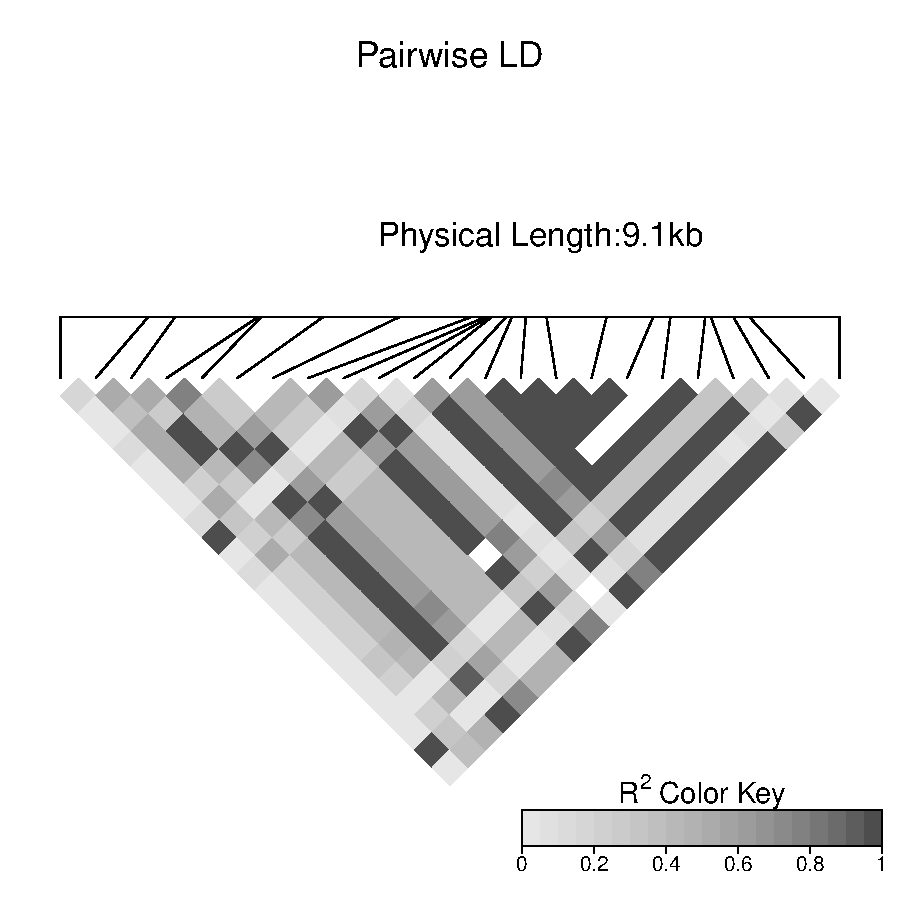
\includegraphics{addTracks-fig1}
\end{center}
\caption{LDheatmap of GIMAP5.CEU data.}
\label{fig:fig1}
\end{figure}

\section{Adding tracks from the UCSC genome browser}

We will add ``UCSC Gene'' and ``Recomb Rate'' tracks 
to Figure~\ref{fig:fig1}. Data for these tracks is downloaded from the
UCSC genome browser using the \texttt{rtracklayer} package.
The genes track is added by the \texttt{LDheatmap.addGenes} function:
\begin{Schunk}
\begin{Sinput}
> llGenes <- LDheatmap.addGenes(ll, chr="chr7", genome="hg18")
\end{Sinput}
\end{Schunk}
It takes several minutes for this function to fetch the necessary data 
from the UCSC genome browser. 
To avoid this download time, users can draw the graphical object (grob) 
stored in \texttt{llGenes} directly (Figure~\ref{fig:fig2}) with 
the commands:
\begin{Schunk}
\begin{Sinput}
> grid.newpage()
> grid.draw(llGenes$LDheatmapGrob)
\end{Sinput}
\end{Schunk}
\begin{figure}
\begin{center}
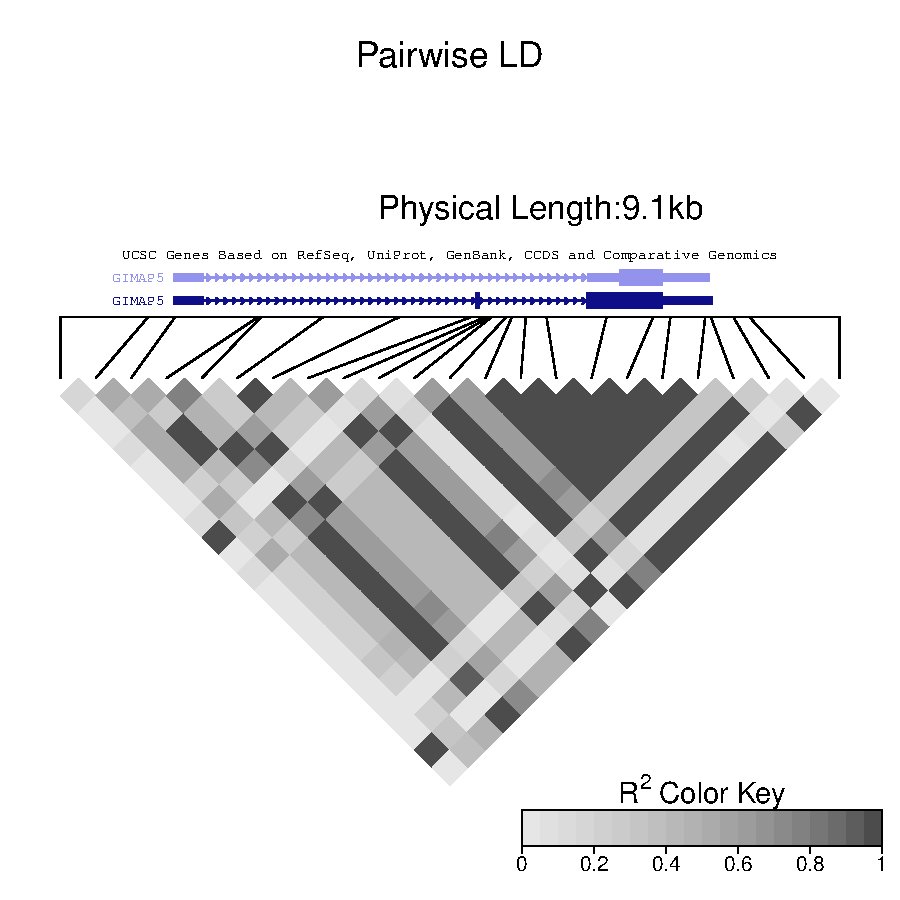
\includegraphics{addTracks-fig2}
\end{center}
\caption{LDheatmap of GIMAP5.CEU data with UCSC Genes track.}
\label{fig:fig2}
\end{figure}

We now add a track that illustrates recombination rates:
\begin{Schunk}
\begin{Sinput}
> llGenesRecomb <- LDheatmap.addRecombRate(llGenes, chr="chr7", genome="hg18")
\end{Sinput}
\end{Schunk}
The result is shown in Figure~\ref{fig:fig3}. Users who wish to 
avoid the download time may draw the
grob from the \texttt{llGenesRecomb} object with the commands:
\begin{Schunk}
\begin{Sinput}
> grid.newpage()
> grid.draw(llGenesRecomb$LDheatmapGrob)
\end{Sinput}
\end{Schunk}
\begin{figure}
\begin{center}
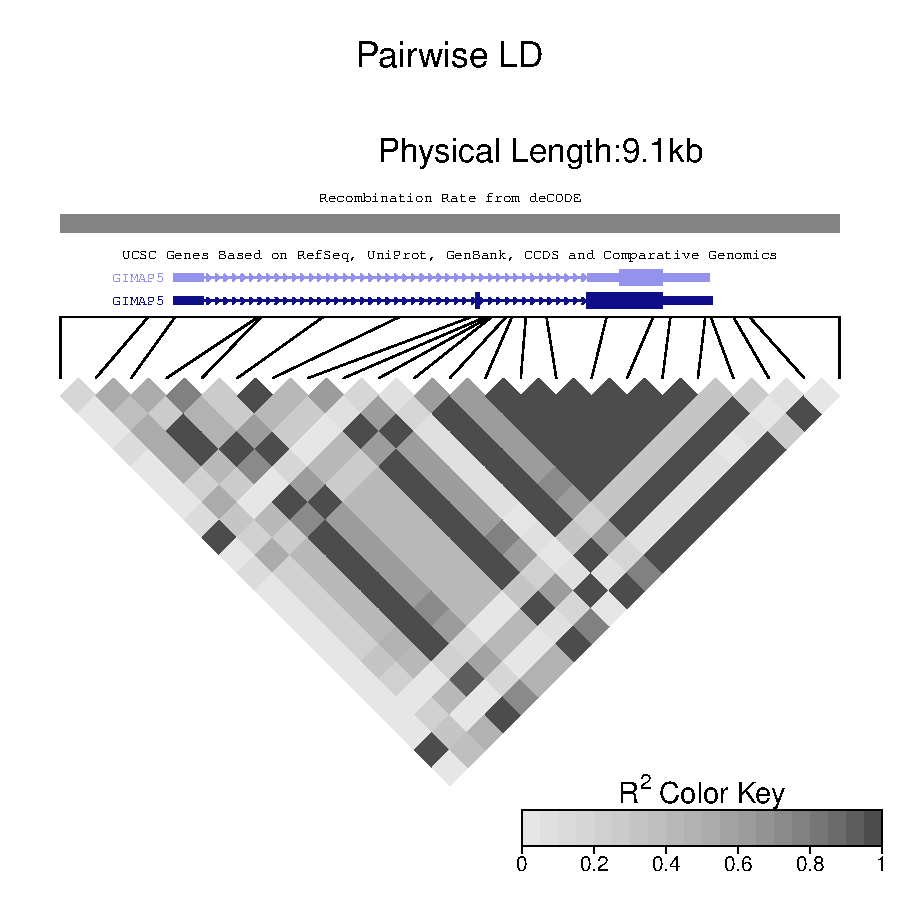
\includegraphics{addTracks-fig3}
\end{center}
\caption{LDheatmap of GIMAP5.CEU data with UCSC Genes and Recomb Rate tracks.}
\label{fig:fig3}
\end{figure}

\section{Adding a scatterplot above the heatmap}

Above the two tracks fetched from the UCSC genome browser
we will superpose a scatterplot depicting the results of
association tests between each SNP in the {\it GIMAP5} gene
and a hypothetical disease.
We create a set of hypothetical p-values that includes
one very small value.
\begin{Schunk}
\begin{Sinput}
> set.seed(1)
> atests<-runif(nrow(GIMAP5.CEU$snp.support))
> names(atests)<-rownames(GIMAP5.CEU$snp.support)
> atests["rs6598"]<-1e-5
\end{Sinput}
\end{Schunk}
A Manhattan plot (scatterplot of the $-\log_{10}$ p-values versus genomic
location of the SNPs) 
can be added to the heatmap as follows:
\begin{Schunk}
\begin{Sinput}
> llGenesRecombScatter<-LDheatmap.addScatterplot(llGenesRecomb,-log10(atests),
+ ylab="-log10(p-values)")